% Fibonacci spiral
% Author: Andrew Mertz
\documentclass{minimal}
\usepackage{amsmath,tikz}
\usepackage{pgfplots}
\pgfplotsset{width=7cm,compat=1.8}
\usetikzlibrary{decorations.markings}
\def\Point{36.9}\usetikzlibrary{backgrounds,calc}


\begin{document}
% I have seen many beautiful depictions of Fibonacci spirals and
% golden spirals. So I thought it would be nice to make a Fibonacci
% spiral in TikZ. I like the look of white on black so here I define a
% black background rectangle.
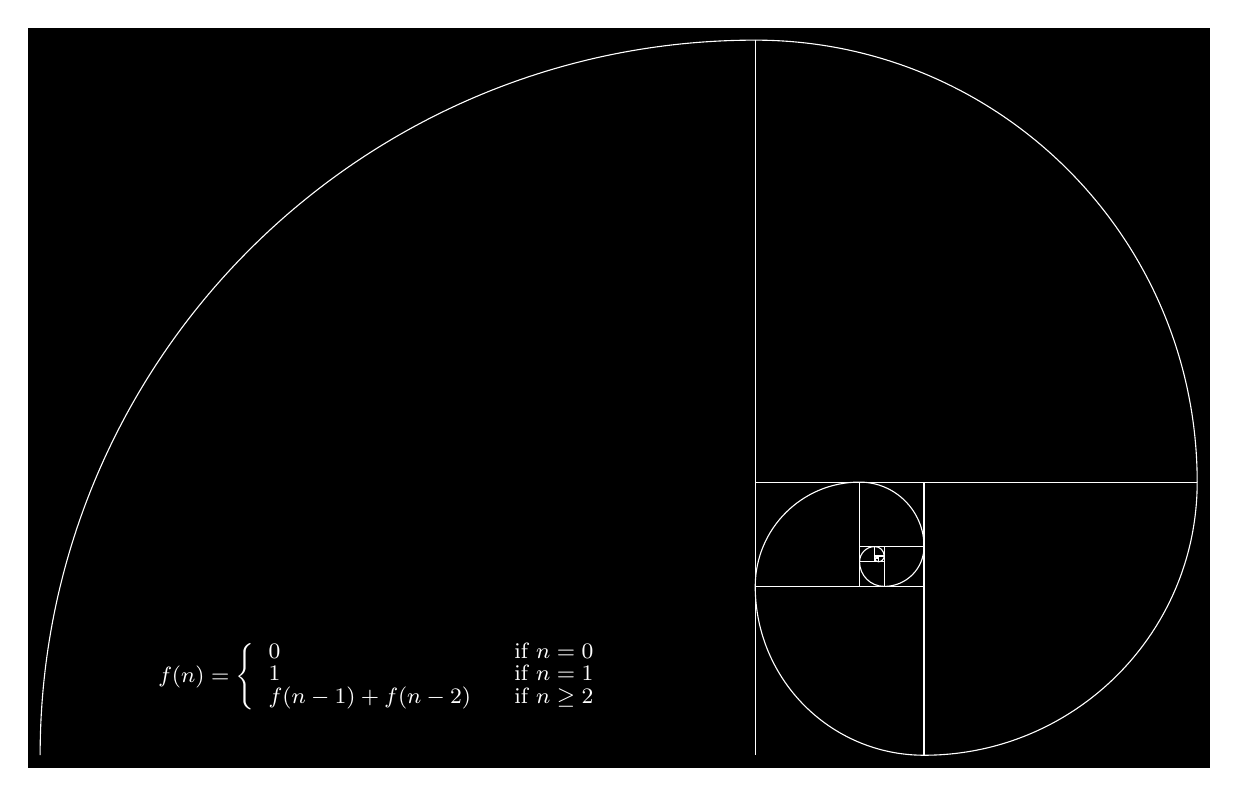
\begin{tikzpicture}[background rectangle/.style={fill=black},
                    show background rectangle] 
  % Create some counters for holding the Fibonacci numbers
  \newcounter{a}
  \newcounter{b}
  \newcounter{temp}

  % Initialize the counters
  \setcounter{a}{0}
  \setcounter{b}{1}

  % The spiral will start at the origin
  \coordinate (0) at (0,0);

  % This loop defines the number of turns in the spiral. Note that we
  % will have to be careful not to overflow our counters or make the
  % spiral too large for TeX to handle. This is easy to do as the
  % Fibonacci sequence grows exponentially.
  \foreach \i in {1,...,18}
  {
    % Get the "name" of the last point on the spiral
    \pgfmathsetmacro{\lastpoint}{\i-1}

    % Compute the angle for this turn of the spiral
    \pgfmathsetmacro{\startangle}{mod(\i-1,4) * 90}

    % Draw this turn of the spiral and remember the point where we end 
    \draw[white] (\lastpoint) arc 
      (\startangle : \startangle + 90 : \value{b}/10.0pt) coordinate (\i);

   % Compute the next Fibonacci number
    \setcounter{temp}{\value{b}}
    \addtocounter{b}{\value{a}}
    \setcounter{a}{\value{temp}}
 }

 % Add some framing for the spiral while at the same time not "boxing"
 % it in. Note that to put a square around each turn of the spiral we
 % could have just used the command \draw[white] (\lastpoint)
 % rectangle (\i); after drawing each turn in the loop above.
 \foreach \i in {1,3,...,17}
 {
   \pgfmathsetmacro{\lastpoint}{\i-1}
   \draw[white] (\lastpoint) -| (\i);
 }

 \foreach \i in {2,4,...,16}
 {
   \pgfmathsetmacro{\lastpoint}{\i-1}
   \draw[white] (\lastpoint) |- (\i);
 }

 \draw[white] (17) -- (17 |- 18);
 
 % Add some text displaying the formula for the Fibonacci numbers
 \node(eq) at ($(18) + (2.5,1)$) 
   [white,text width = 2cm,font=\fontsize{8}{8}\selectfont] {
   \begin{displaymath}
     f(n) = \left\{
       \begin{array}{lr}
         0 & \text{~~if } n = 0\\
         1 & \text{~~if } n = 1\\
         f(n-1) + f(n-2) & \text{~~if } n \geq 2\\
      \end{array}
     \right.
   \end{displaymath}
  };
\end{tikzpicture}

\begin{tikzpicture}[background rectangle/.style={fill=black},
                    show background rectangle, x=1pt, y=1pt, size=0.125]
 % Compute the golden ratio
  \pgfmathsetmacro{\goldenRatio}{(1+sqrt(5)) / 2}

  % Compute the angle between the tangent and radial line 
  \pgfmathsetmacro{\offset}{rad(atan(2*ln(\goldenRatio)/pi))};

  % Plot the spiral using the parametric form of a logarithmic spiral
  % (a e^{b t} cos(t), a e^{b t} sin(t)). In this case a = 1 and b = 2
  % ln((1+sqrt(5)) / 2) / pi. There can be a slight gap between the
  % last line segment and the end of the plot. Having a large sample
  % size reduces the gap.
  \draw[very thick,white,domain=\offset:\offset+14*pi/2,
       smooth,samples=600,variable=\t] plot
   ({pow(\goldenRatio, 2 * \t / pi) * cos(\t r)},
    {pow(\goldenRatio, 2 * \t / pi) * sin(\t r)}) 
   coordinate(end);

  % Remember the start of the spiral
  \coordinate (0) at 
    ({pow(\goldenRatio, 2 * \offset / pi) * cos(\offset r)},
     {pow(\goldenRatio, 2 * \offset / pi) * sin(\offset r)});

 % This loop draws the line segments
  \foreach \i in {1,...,14}
  {
    % Get the "name" of the last point on the spiral
    \pgfmathsetmacro{\lastpoint}{\i-1}

    % Compute the start angle for this turn of the spiral
    \pgfmathsetmacro{\angle}{\i * pi / 2  + \offset}

   \draw[very thick,white] (\lastpoint) --
     ({pow(\goldenRatio, 2 * \angle / pi) * cos(\angle r)},
      {pow(\goldenRatio, 2 * \angle / pi) * sin(\angle r)})
     coordinate (\i);
  }

  % Add some text displaying the formula for the parametric form of the
  % spiral
   \node(eq) at ($(14) + 5*(\goldenRatio cm,1cm)$) 
     [white,text width=2cm,font=\fontsize{30}{30}\selectfont,
      anchor=north west] {
     \begin{displaymath}
       \begin{array}{llll}
         x&(\theta) = \phi^{\frac{2\theta}{\pi}}&\cos&(\theta)\\
         y&(\theta) = \phi^{\frac{2\theta}{\pi}}&\sin&(\theta)\\
       \end{array}
     \end{displaymath}
  };
\end{tikzpicture}


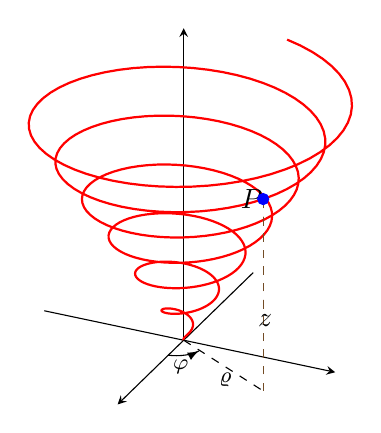
\begin{tikzpicture}
  \begin{axis}[
    view       = {-25}{-25},
    axis lines = middle,
    zmax       = 60,
    height     = 8cm,
    xtick      = \empty,
    ytick      = \empty,
    ztick      = \empty
  ]
  \addplot3+ [
    ytick      = \empty,
    yticklabel = \empty,
    domain     = 0:14.7*pi,
    samples    = 400,
    samples y  = 0,
    mark       = none,
    thick,
    red,
  ]
  ( {x*sin(0.28*pi*deg(x))},{x*cos(0.28*pi*deg(x)},{x});
  \addplot3+ [
    mark options = {color=blue},
    mark         = *
  ] 
  coordinates {({\Point*sin(0.28*pi*deg(\Point))},
    {\Point*cos(0.28*pi*deg(\Point)}, {\Point})};
  \addplot3+ [
    domain    = 0:12*pi,
    samples   = 100,
    samples y = 0,
    mark      = none,
    dashed,
  ]  
  ( {\Point*sin(0.28*pi*deg(\Point))}, {\Point*cos(0.28*pi*deg(\Point)}, {x} );
  \addplot3[
    mark=none,
    dashed
  ]
  coordinates {(0,0,0) ({\Point*sin(0.28*pi*deg(\Point))},
    {\Point*cos(0.28*pi*deg(\Point)}, {0})};
  \draw[
    radius = 80,
    decoration = {
      markings,
      mark= at position 0.99 with {\arrow{latex}}
    },
    postaction=decorate
  ] 
  (axis cs:0,10,0) arc[start angle=80,end angle=14] (axis cs:14,0,0);
  \node at (axis cs:20,0,30) {$P$};
  \node at (axis cs:24,0,7) {$z$};
  \node [font=\footnotesize] at (axis cs:20,17,0) {$\varrho$};
  \node [font=\footnotesize] at (axis cs:6,15,0) {$\varphi$};
  \end{axis}
\end{tikzpicture}
\end{document}
% LocalWords:  tikzpicture eq lr TikZ
